\chapter{State of Art}
\label{chap:state-of-art}
\textit{Introduction of the state of art}

\clearpage
\section{Mental illness: Eating Disorders}

In the Section \ref{sec:context}, we have understood in general terms what are Mental Health and Eating Disorders and its importance nowadays in society. It has been key to dive deep into these concepts for projecting and posing this Master Thesis and for understanding what challenges and problems we will face while tackling the Eating Disorder topic.

The Biopsychosocial model by Dr. George Engel and John Romano(1977) helps to have a broad picture of the Eating Disorders because it analyses and breaks down the topic of the Eating Disorders into smaller pieces.

%MODEL OF MENTAL HEALTH ------------------------------------
% https://www.open.edu/openlearn/science-maths-technology/exploring-the-relationship-between-anxiety-and-depression/content-section-2
% 1 - INTERESTING BIOPSYCHOSOCIAL model for Mental Health: https://www.careershodh.com/what-is-biopsychosocial-model-of-health/
% BIOPSYCHOSOCIAL EDs: https://withinhealth.com/blog/posts/what-causes-an-eating-disorder-a-biopsychosocial-perspective
% https://www.researchgate.net/publication/8330681_Cognitive-Behavioral_Theories_of_Eating_Disorders

The framework proposed by Dr. George Engel and John Romano in 1977 called biopsychosocial model~\cite{WhatisBi40:online} considers biological, psychological and social aspects and their interactions to understand health, illness and health care delivery. This model is both a practical clinical guide and a philosophy of clinical care. 

The latter is concerned with understanding how suffering, disease and illness are affected at different levels from the molecular to the societal. At the practical level, it is a way of looking at the subject's experience as a key element in human care, accurate diagnosis and health outcomes.% Understanding this model will help us to address the main issue raised by this work, the diagnosis of mental illness and in particular Eating Disorders.

As can be seen in Figure \ref{fig:biopsychosocial}, the aforementioned model has 3 distinct parts, the biological, which includes physiological pathologies; the psychological, under which fall emotions, thoughts and behaviours such as distress, fear, avoidance, etc.; and the social, which includes cultural, socio-economic and socio-environmental factors such as circumstances that the subject may experience at work or in the family.

\begin{figure}[!htp]
    \centering
    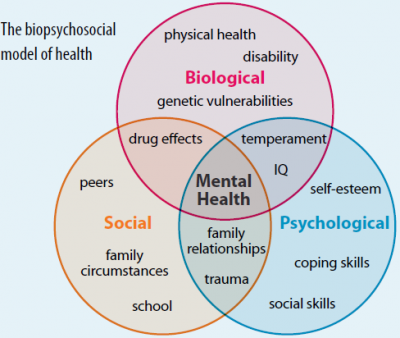
\includegraphics[scale=0.65]{img/state-of-art/biopsychosocial model.png}
    %\begin{minipage}{1}
    %\footnotesize
    %\emph{YOUR NOTES}
    %\end{minipage}
    \caption{Biopsychosocial Model of Health~\cite{Biopsych52:online}.}
    \label{fig:biopsychosocial}
\end{figure}

%ASSOCIATION WITH MODEL OF EDs------------------------------------
%\section{Model of mental illness and ED}

In this Master Thesis we have focused on mental illnesses related to Eating Disorders, so we have proceeded to do a search on the modelling of these problems in this Biopsychosocial model in order to attack the topic that interests us most, as mentioned above, the diagnosis. According to studies carried out by experts~\cite{WhatCaus58:online}, the aspects marked in Table~\ref{tab:biopsychosocialForEDs} have potential to be included in each level of the model.

\begin{table}[]
\begin{tabular}{|c|c|c|}
\hline
\textbf{Biological} & \textbf{Psychological} & \textbf{Social} \\ \hline
\begin{tabular}[c]{@{}c@{}}Family and personal history \\ of dieting and overeating\end{tabular} & Perfectionism & \begin{tabular}[c]{@{}c@{}}Weight-related teasing \\ and bullying\end{tabular} \\ \hline
High parental control & Novelty-seeking traits & \begin{tabular}[c]{@{}c@{}}Internalizing body image ideals \end{tabular} \\ \hline
\begin{tabular}[c]{@{}c@{}}Parental substance \\ use disorder\end{tabular} & Neuroticism & Separation from parent \\ \hline
\begin{tabular}[c]{@{}c@{}}Type I diabetes \\ (insulin-dependent)\end{tabular} & Conduct disorder & Weight stigma \\ \hline 
& Physical or sexual abuse & \begin{tabular}[c]{@{}c@{}}Acculturation, or assimilation \\ into Western culture\end{tabular} \\ \hline
& \begin{tabular}[c]{@{}c@{}}High levels of body \\ image dissatisfaction\end{tabular} & Intergenerational trauma\\ \hline
& \begin{tabular}[c]{@{}c@{}}Personal history of \\ an anxiety disorder\end{tabular} & \\ \hline
\end{tabular}
\caption{Biopsychosocial model for Eating Disorders}
\label{tab:biopsychosocialForEDs}
\end{table}


These indicators potentially show, if present in a subject, the possible suffering of an Eating Disorder, although the final diagnosis must be made by a professional to confirm and start treatment. We would also like to emphasise the process of the medical diagnostic of the main three Eating Disorders: Anorexia Nervosa, Bulimia Nervosa and Binge Eating, which we are tackling hereafter.

% TALK ABOUT METHODS TO DIAGNOSE EDs--------------------------------------------------------
% https://www.aafp.org/pubs/afp/issues/2003/0115/p297.html
%https://books.google.es/books?hl=es&lr=&id=mM7SAgAAQBAJ&oi=fnd&pg=PA155&dq=diagnosis+of+eating+disorder&ots=GA8hyKuevS&sig=sJShW_lqCcRK1S43G2mtpT-ihRg#v=onepage&q=diagnosis%20of%20eating%20disorder&f=false
% https://journals.sagepub.com/doi/abs/10.1177/070674379504000805

As experts have discussed~\cite{pritts2003diagnosis}, a number of problems can mask the disorder and should be considered before a diagnosis of an Eating Disorder is made, such as hyperthyroidism, malignancy, inflammatory bowel disease, immunodeficiency, malabsorption, chronic infections, Addison's disease, and diabetes. A preoccupation with weight is observed in most patients with a health problem that leads to eating problems, but it is the patients who are diagnosed with an Eating Disorder who manifest a distortion of body image and want to be underweight.

According to the paper written by Garfinkel in 1995~\cite{garfinkel1995views}, several criteria for classifying and diagnosing Anorexia Nervosa, Bulimia Nervosa and Binge-Eating Disorder are defined.


\myparagraph{Anorexia Nervosa}
Following the scientific papers, Anorexia Nervosa is the \textit{``eating disorder, universally associated with emaciation and commonly accompanied by marked increases in physical activity''}~\cite{bulik2005anorexia}. The criteria for diagnosis this illness is defined as follows.
\begin{itemize}
    \item Refusal to maintain body weight at or above a minimally normal weight forage and height, e.a., weight loss leading to maintenance of body weight less than 85\% of that expected; or failure to make expected weight gain during a period of growth, leading to body weight less than 85\% of that expected.
    \item Intense fear of gaining weight or becoming fat, even though underweight.
    \item Disturbance in the way in which one's body weight or shape is experienced, denial of the seriousness of current low body weight, or undue influence of body shape and weight on self-evaluation.
    \item In post-menarcheal females amenorrhea, i.e., absence of at least 3 consecutive menstrual cycles. (A woman is considered to have amenorrhea if her periods occur only following hormone, e.o., estrogen administration.)
\end{itemize}

It has two sub types, which are i)Binge-Eating/Purging Type, in which the individuals have purging or binge-eating behaviour; ii) Restricting type, in which the subjects who suffer it limit calorie intake.


\myparagraph{Bulimia Nervosa}
This Eating Disorder is marked by episodes of binge eating followed by purging behaviors to prevent gain, as marked in the paper from Dr. Mehler~\cite{mehler2003bulimia}. In contrast to anorexia nervosa, which is characterized by a weight that is less than 85 percent of the normal value, most persons with bulimia are of normal weight. The criteria defined for diagnosis is defined in DSM-IV (Diagnostic and Statistical Manual)~\cite{widiger1997dsm} as follows.
\begin{itemize}
    \item Recurrent episodes of binge eating. An episode of binge eating is characterized by both of the following:
    \begin{itemize}
        \item Eating, in a discrete period of time (e.g., within any 2-hour period), an amount of food that is definitely larger than most people would eat during a similar period of time and under similar circumstances.
        \item A sense of lack of control over eating during the episode (e.g., a feeling that one cannot stop eating or control what or how much one is eating).
    \end{itemize}
    \item Recurrent inappropriate compensatory behaviour in order to prevent weight gain, such as: self-induced vomiting; misuse of laxatives, diuretics or other medications; fasting; or excessive exercise.
    \item The binge eating and inappropriate compensatory behaviours both occur, on average, at least twice a week for 3 months.
    \item Self-evaluation is unduly influenced by body shape and weight.
    \item The disturbance does not occur exclusively during episodes of anorexia nervosa.
\end{itemize}

As Anorexia Nervosa, it has also two sub types: i) Purging type, when the person has regularly in self-induced vomiting or the misuse of
laxatives, diuretics or enemas; ii)Nonpurging Type, when the patient is using inappropriate compensatory behaviours like fasting or exercise.

\myparagraph{Binge-Eating Disorder}
This disorder was a new introduction in the DSM-IV, although it is not a formal diagnosis within the DSM-IV, but in day-to-day clinical practice the diagnosis seems to be generally accepted. People with the BED-syndrome have binge eating episodes as do subjects with bulimia nervosa, but unlike the latter they do not engage in compensatory behaviours, according to what Dingemans states~\cite{dingemans2002binge}. The criteria to follow in order to diagnose it is as follows.
\begin{itemize}
    \item Recurrent episodes of binge eating. An episode of binge eating is characterized by both of the following:
    \begin{itemize}
        \item Eating, in a discrete period of time (e.c., within any 2-hour period), an amount of food that is definitely larger than most people would eat in a similar period of time under similar circumstances.
        \item Asense of lack of control over eating during the episode (e.g., a feeling that one cannot stop eating or control what or how much one is eating).
    \end{itemize}
    \item The binge-eating episodes are associated with 3 (or more) of the following:
    \begin{itemize}
        \item Eating much more rapidly than normal.
        \item Eating until feeling uncomfortably full.
        \item Eating large amounts of food when not feeling physically hungry.
        \item Eating alone because of being embarrassed by how much one is eating.
        \item Feeling disgusted with oneself, depressed or very guilty after overeating.
    \end{itemize}
    \item Marked distress regarding binge eating is present
    \item The binge eating occurs, on average, at least 2 days a week for 6 months.
    \item The binge eating is not associated with the regular use of inappropriate compensatory behaviours (e.g., purging, fasting, excessive exercise) and does not occur exclusively during the course of anorexia nervosa or bulimia nervosa.

\end{itemize}

With all of the above in mind, the aim of this project is to design and implement a system that will help diagnose these illnesses, serving as a complementary tool and as an orientation aid to the medical methods used today, as these are irreplaceable and also necessary in mental illnesses as important as those discussed above.



\section{Text Classification}
This Master Thesis is based on text classification methods. These techniques allow us to identify and extract information from existing resources using Machine Learning. Using them, we can determine what a person thinks about a particular topic, in our case Eating Disorders. This position can be a value judgement, a communication intention or an emotional state.

\subsection{Machine Learning}
As mentioned before, text classification is based on machine learning, which has different definitions, the first being the one provided by Arthur Samuel in 1959 which defines this concept as \textit{``Field of study that gives computers the ability to learn without being explicitly programmed''}~\cite{samuel1959some}.
Over the years as it has undergone a great evolution, having a newest definition such as the one given in~\cite{el2015machine}: \textit{``Machine learning is an evolving branch of computational algorithms that are designed to emulate human intelligence by learning from the surrounding environment''}.

There are different techniques encompassed within Machine Learning in order to better adapt to the use case study on each occasion. T.Ayodele recounts that there are specifically six types~\cite{ayodele2010types}: Supervised Learning, Unsupervised Learning, Semi-supervised Learning,  Reinforcement Learning, Transduction and Learning to learn, but we will focus on the most relevant ones which are Supervised , Unsupervised and Reinforcement Learning.
\myparagraph{Supervised Learning}
Method used commonly in classification problems since the principal goal is to the computer to learn a classification system that we have already created. In general, this type of learning is optimal for any problem where a classification of elements is needed and it is easy to define. 

These desired classification could be for both discrete(e.g. an integer, a label or a boolean) and continues values, and each case we are talking of \textit{Classification} or \textit{Regressive} problems, and the two of them are tackled in a similar way. In the Figure \ref{fig:supervised-learning} we can see an example for better understanding the difference among the described types.

\begin{figure}[!h]
    \centering
    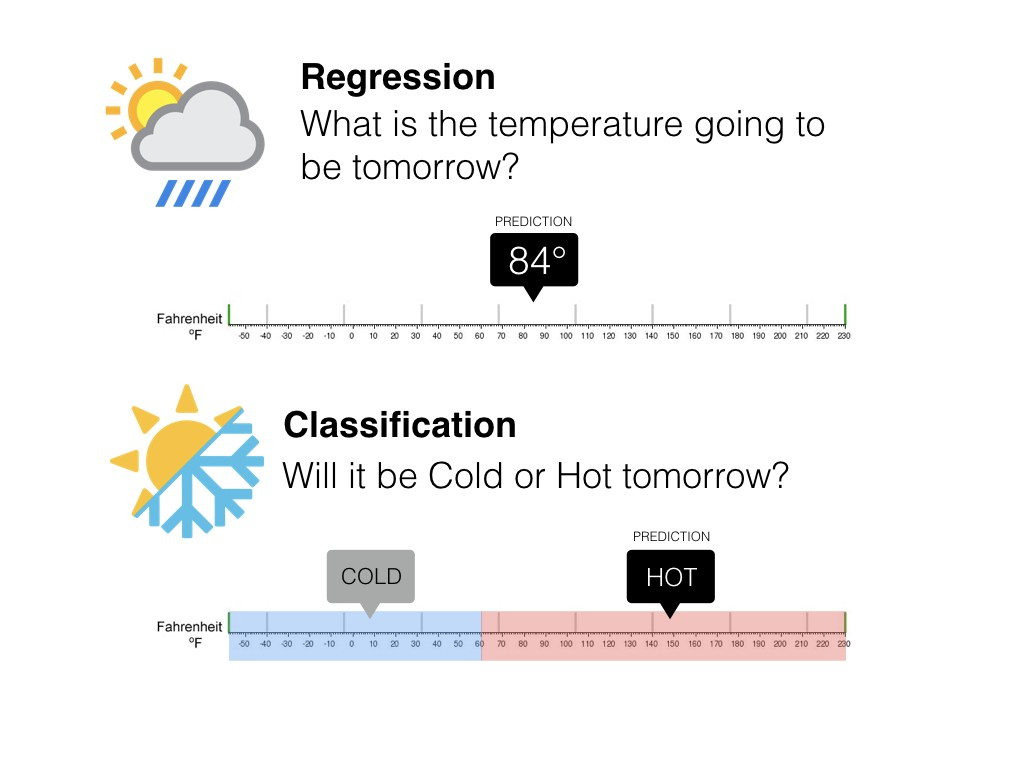
\includegraphics[scale=0.27]{img/state-of-art/supervised-learning.jpeg}
    \caption{Different types of Supervised Learning}
    \label{fig:supervised-learning}
\end{figure}

Supervised Learning is the most common technique in Neural Networks and Decision Trees, since these are highly dependent on the information provided by already determined classifications.
%% SE PODRIA EXTENDER SUPERVISED LEARNING

\myparagraph{Unsupervised Learning}
This type of learning aims to induce patterns in the observed data without having any knowledge about them, which makes the task much more complicated a priori. The most commonly used technique in this case is clustering, which is a data mining technique that groups elements by similarities and induces classifications. These algorithms are used to process unclassified objects into information structures. There are several types of clustering, such as exclusive, overlapping, hierarchical, and probabilistic clustering~\cite{WhatisUn52:online}.

%% HABLAR DE DIMENSIONALITY REDUCTION???

An example of an unsupervised algorithm is the so-called k-means clustering, which aims at partitioning a set of n observations into k groups, where each observation belongs to the group whose mean value is closer to the nearest.
\myparagraph{Reinforcement Learning}
One of the most important types of learning is Reinforcement Learning, which is defined in~\cite{sutton2018reinforcement} as follows: ``Reinforcement learning is learning what to do-how to map situations to actions-so as to maximize a numerical reward signal. The learner is not told which actions to take, but instead must discover which actions yield the most reward by trying them.''

This learning is rather empirical, in that each decision intelligence makes is evaluated and rewarded positively or negatively depending on the success of that decision. This is why it often takes many attempts to bring the learning to the desired accuracy.\\

Now that the basics have been understood and the different paths that can be taken using Machine Learning have been explained, we are proceeding to discuss the models that we are going to use for performing the Machine Learning.

\subsection{Machine Learning models}
An important part of this project is the model we use for making the prediction. We have conducted a research and an analysis for getting more knowledge on the available tools that we can have for reaching our objective.

Before starting, it is important to mark the kinds of the algorithms that have been checked. One type of them are the algorithms that have been used for some time now that we call `Traditional Models' which include the Random Forest, SVM and Logistic Regression; and the  BERT models which are pretrained models that adapt to the data you have and are based on Neural Networks.

In this subsection we are going to break them out for getting more information on them and their functioning.

\subsection{Traditional Models}
In this project, we call traditional models those models that have not been pre-trained and are historically more consolidated in the field of Machine Learning and Artificial Intelligence, despite this being a relatively new and booming field.

\subsubsection{Random Forest}
Random Forest~\cite{breiman2001random} is a decision tree-based Machine Learning algorithm used for classification or regression of data by constructing many decision trees when training the model. These models are sampled independently and with the same distribution for all the members. In the case of classification, the output tree is the class selected by the largest number of trees, as in our case. A representation of it can be seen in the Figure~\ref{fig:random-forest}.

\begin{figure}[!htp]
    \centering
    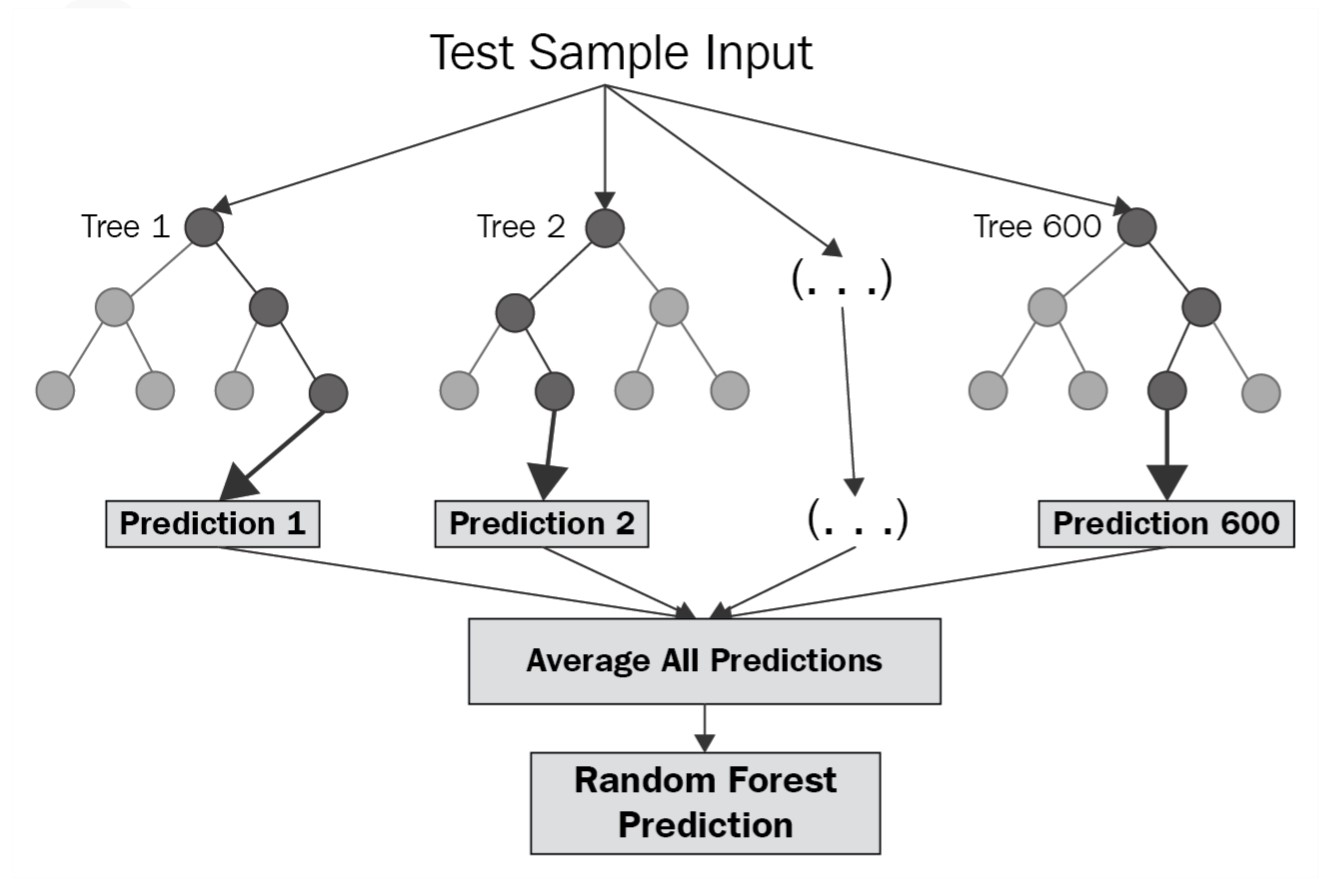
\includegraphics[scale=0.3]{img/detection/random-forest.jpg}
    \caption{Random Forest model representation}
    \label{fig:random-forest}
\end{figure}

The generalization error for these forest converges to a limit with the increase of the size of this forest. This errror depends on the strength of the singular trees and the correlation among them. This algorithm corrects the flaw in decision trees of overfitting the training set, i.e. overtraining a learning algorithm so much that it is only effective under very specific conditions, those of the training data.

\subsubsection{SVM}
The Support Vector Machine algorithm~\cite{chauhan2019problem}, also known as SVM, is an optimal margin based classification technique in Machine Learning. The objective of this is to find a hyperplane that best separates two different classes of data points,\textit{ i.e.} with the widest margin between the two classes. 

It is a binary linear classifier which has been enhanced to support non-linear data using various Kernels. SVM is continuously improving since its invention and the experts have pose different formulations for solving SVM. 

\begin{figure}[!htp]
    \centering
    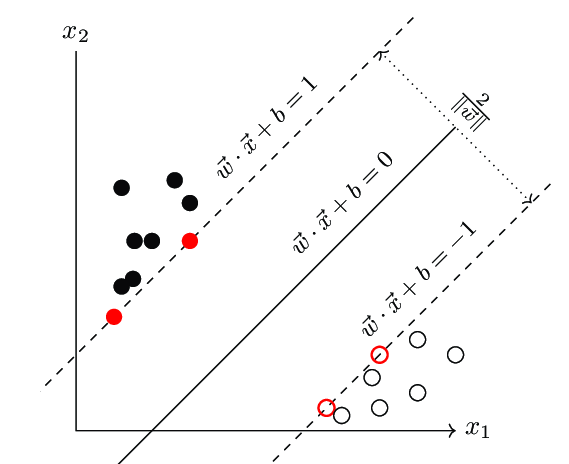
\includegraphics[scale=0.4]{img/detection/SVM.png}
    \caption{SVM model representation}
    \label{fig:SVM}
\end{figure}

The margin we raised before is defined as the maximum width of the region parallel to this hyperplane that has no interior data points. This algorithm only works on problems that allow linear separation, maximising the aforementioned margin as it can be seen in Figure~\ref{fig:SVM}.

\subsubsection{Logistic Regression}
Logistic regression is one of the most important statistical and data mining techniques for analysis and classification for datasets that are binary and proportional~\cite{maalouf2011logistic}. This model is within supervised learning and is used to predict the categorical dependent variable given a set of independent variables. This predicted output can take both categorical and discrete values and is used for classification problems. In this regression, an attempt is made to fit the values within an ``S" shaped logistic function that predicts between two maximum values, either 0 or 1 as can be seen in Figure~\ref{fig:LogisticRegression}.

\begin{figure}[!htp]
    \centering
    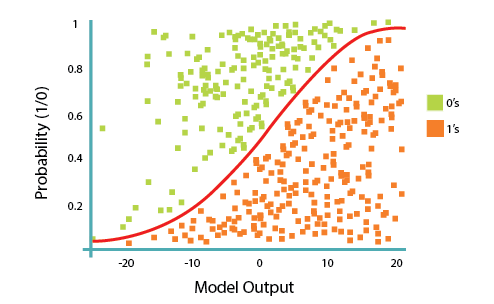
\includegraphics[scale=0.6]{img/detection/LogisticRegression.png}
    \caption{Logistic Regression representation model}
    \label{fig:LogisticRegression}
\end{figure}



\subsection{BERT Models}
%% METER ARQUITECTURA MODELS

After explaining the traditional models as we have called them in the present project, in which we had a mathematical algorithm that had to be trained to optimise the models to subsequently make the predictions, we are going to explain the BERT models (Bidirectional Encoder Representations from Transformers). 

BERT models~\cite{acheampong2021transformer} are pre-trained and open source machine learning techniques based on neural networks for NLP developed by Google in 2018. These algorithms have been used in the company's search engine since 2019. BERT makes use of Transformer, an attention mechanism that learns the contextual relationships between words and includes two different mechanisms, an encoder that reads the input text and a decoder that produces a prediction. This encoder is the necessary element, because BERT's goal is to generate a language model.

BERT models can be used for a number of different linguistic tasks by adding only a small layer to the core model. In classification tasks, as is the case in this project and in sentiment analysis, they are performed in a similar way to Next Sentence Prediction (NSP) techniques, by adding a classification layer on top of the output of the token transformer (CLS)~\cite{BERTExpl89:online}.

In the NSP training process, the model is provided with pairs of sentences as input and learns whether the second sentence of the pair is the next sentence in the original document to learn about the context. 50\% of the input sentence pairs are the subsequent sentences in the original document and the other 50\% are randomly chosen and disconnected sentences. In order to process the input text the following steps are needed to be performed, as it can be seen in Figure~\ref{fig:BERTinput}.

\begin{enumerate}
    \item A CLS token and a SEP token are inserted at the beginning and end of each sentence respectively.
    \item A phrase embedding indicating phrase A or phrase B is added to each token.
    \item A positional inlay is added to each token to indicate its position in the sequence.
\end{enumerate}

\begin{figure}[!htp]
    \centering
    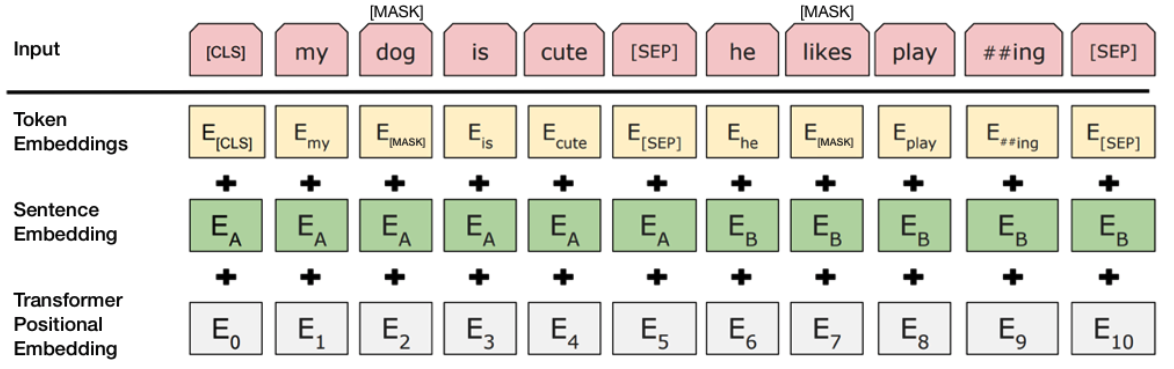
\includegraphics[scale=0.35]{img/detection/BERTinput.png}
    \caption{BERT input processing in NSP}
    \label{fig:BERTinput}
\end{figure}
Once the input text has been pre-processed, to make the prediction of the second sentence over the first, the following is needed.

\begin{enumerate}
    \item Introducing the sequence to the Transformer model.
    \item The output of the [CLS] token is transformed into a 2x1 vector using one of classification.
    \item Calculate the probability with softmax or normalised exponential function.
\end{enumerate}

BERT models have also variants which provide different approaches optimised for specific use cases. In our case, we have investigated about roBERTa and concretely Mental roBERTa, which seeks to optimize BERT in various methodological parameters and it is focused on mental health problems. It helps to investigate hyperparametes such as larger pre-training datasets, batch sizes or text encoding.

A remark should be put as well on mBERT, a model which is based on BERT trained with a big corpus that support a large amount of languages. \\

So now that the basics and the models have been discussed in the chapter, we are proceeding to talk about the Text Classification Techniques that need to be implemented for putting our project to work.
\subsection{Text Classification Techniques}

To understand the different problems of Text Classification it is important to review the architecture of this, as can be seen in Figure \ref{fig:text-clasification-architecture}, which will generally found in almost all text classification cases conducted today. It is divided into 5 parts described below:


\begin{itemize}
    \item Corpus: input of documents in any format (XML, JSON, CSV, PDF, etc.)
    \item Document processing: documents are preprocessed using linguistic tools like tokenization, part of speech tagging, lemmatization, stemming, etc.
    \item Lexicons and linguistic resources: supporters of the whole architecture
    \item Document analysis: key part where the documents that are preprocessed are interpreted using the linguistic resources
    \item Scores: presentation of the results after analysing documents, using visualization tools.
\end{itemize}


\begin{figure}[!htp]
    \centering
    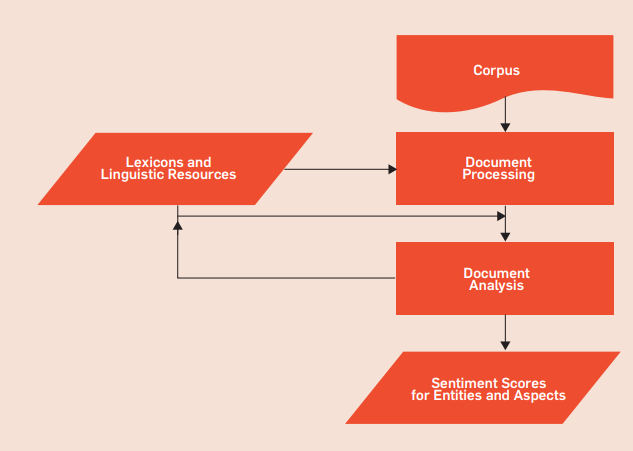
\includegraphics[scale=0.75]{img/state-of-art/text-classification-architecture.png}

    \caption{Generic text classification system architecture~\cite{feldman2013techniques}}
    \label{fig:text-clasification-architecture}
\end{figure}

% TECNICAS DE ANALISIS DE SENTIMIENTOS ----------------------------------------
% https://dl.acm.org/doi/abs/10.1145/2436256.2436274?casa_token=lqpbt-cBaHYAAAAA:x2yhJourTm6uZJepBIzElTx3v759Iv2UVKWlQi1CJJEsUy1qxoJfzYHWRs6XGJy9onXToAkI-Ow2kg

Knowing this architecture, there are some problems to solve while performing the text classification that the expert have spotted as key for the success of the learning~\cite{feldman2013techniques}. There are different ways of approaching a problem of analysis such as this Master Thesis, generating different approaches that must be know before digging into the technical part. We will discuss now the problems of document-level classification, sentence-level classification and lexicon acquisition.

\myparagraph{Document-level classification}
This form is the simplest of all text classification, which assumes that the document itself has a value judgement on a main subject expressed by the author of the subject. This approach can be tackled with both supervised and unsupervised learning. The first one takes the assumption that there is a finite set of classes(e.g. the simplest case, positive and negative) into which the document must be classified having training data for each one. The unsupervised approach is based on determining the semantic orientation (SO) of certain phrases in the document.

Researchers have found good results when each document is represented as a simple bag of words, meanwhile the unsupervised approach has worked well in English but it is lacking linguistic resources when switching to other major spoken languages such as Chinese and Spanish and thus, throwing worse results.

\myparagraph{Sentence-level classification}
This approach is considering that a document can contain different opinions about the same subjects, so when we need to have a deeper zoom for analyse it and move to the sentence level this it the approach that is more adequate. It consist in assuming that each sentence has a different opinion, and then it can be relaxed analysing different phrases and collect them into groups for then apply the machine learning techniques.

%\myparagraph{Aspect-based classification}
%Aspect-based classification opens the spectrum of entities to which the analysis is done. While the previous two work when the author refers to one entity, in many cases the people talk about different attributes that need to be consider since the opinion about them can be different. This approach is defined as \textit{``research problem that focuses on the recognition of all expressions within a given document and the aspects to which they refer''}.

%There are two ways of handling kind of analysis, the classical approach of this is extracting all noun phrases (NPs) and keep the ones whose frequency is higher an experimentally determined threshold, and the other one is use a phrase dependency parser that uses known expressions to search for additional aspects.

%\myparagraph{Comparative classification}
%Usually the authors provide their opinion about a subject through the comparison with other subjects so the goal of this technique is to assess which sentence contains a comparative opinion and extract the preferred entities in each. Researchers in this field have found the most common words that we use for the 98\% of the cases so with them we can start separating the comparison and analyse them properly~\cite{jindal2006identifying}.

\myparagraph{Lexicon Acquisition}
This part is usually the most crucial resource for the text classification algorithms and there are three ways to acquire it: i) manually, in which people code the lexicon by hand; ii) dictionary-based approaches in which with seed words the lexicon is expanded using external resources; iii) corpus-based approaches where a set of seed words the lexicon is expanded by using a large corpus of documents.\\

These are the challenges that can be found when working with Text Classification that must be known before going into the technical details. After in this Thesis we will talk about how do we tackle them and the resolution of the conflicts that we have found, but before, we want to shed light on the text classification already carried out on social networks as this will be our case study so, in the next subsection we will expose them.




\section{Related work}
\label{sec:studies}

%https://dl.acm.org/doi/pdf/10.1145/3366030.3366058
%https://www.jmir.org/2015/11/e256/
% INTERESANTE COMPARACION BERT MODEL: https://medinform.jmir.org/2022/2/e34492/

In this Master Thesis thesis we are going to use text classification in social networks as detailed in Section \ref{sec:goals} so we have made a review of what is already implemented in order to build our system taking into account previous contributions.

One study~\cite{oksanen2015pro} analysed videos and comments from YouTube channels related to pro-anorexia and anti-anorexia communities. It was found in this study that, although pro-anorexia videos are widespread on the platform, videos that promote help and oppose the community are more popular, having more positive comments and feedback. This makes anti-pro-anorexia communities into helping forces that professionals should give more support to.

Another scientific paper~\cite{benitez2022traditional} mentions other models which have also importance in the field. They are the so-called Bidirectional Encoder Representations from Transformer or also known as BERT models, which we will talk about next. This study focused on finding Machine Learning models capable of efficiently categorising tweets about Eating Disorders, the main objective of our system.

For this purpose, tweets related to Eating Disorders were collected and a subset of 2000 tweets were classified into different categories that would help to better understand the collected material. Traditional and deep learning machine learning methods were used and then evaluated with accuracy, F1 score and computational time. 

Among the traditional methods, Random Forest was used, which will be discussed below, and, as reported in the paper, BERT models had the best score of all the techniques used, ranging from 71.1\% to 86.4\%, although they took the longest computation time. Methods such as Recurrent Neural Networks or Bidirectional long short-term memory were also used, scoring better than Random Forest but without reaching the accuracy of the BERT models.

% METER ALGUN PAPER MAS??? SOLO INCLUIDOS 2


Knowing all this, we embark on the implementation of the application we want to realise, using everything discovered in these publications mentioned during the current chapter. To do this, we need a basic knowledge of the tools that will help us to shape our system, which are detailed below. 


\section{Enabling Technologies}
In this Section we will discuss the technologies that support this Master Thesis, without which its implementation would not have been possible. We will review the part that has contributed to Machine Learning, through the use of the Python language and different algorithms implemented in its libraries, as well as the part that has been developed for the server with Flask and the web application implemented in Dart language through Flutter.

% Parte de enabling technologies con python y modelos???
\subsection{Machine Learning Technologies}
To work with the Machine Learning in this Master Thesis, Python has been used as it is a language that supports this technology very well with its pre-established libraries and comes with many models already implemented, very easy to use through the use of Jupiter Notebooks.

\subsubsection{Python and extensions}
Python~\cite{Welcomet44:online} is a programming language created in the late 1980s by Guido van Rossum at the Centre for Mathematics and Informatics (CWI, Centrum Wiskunde \& Informatica) in the Netherlands as a descendant of the ABC programming language. As a curiosity, the name language comes from its creator's fondness for the British comedians Monty Python. It is a high-level interpreted language whose focus is on the readability of the code, as well as being a multi-paradigm language (it partially supports object-oriented, imperative programming and to a lesser extent functional programming). It is a dynamic(a variable can take on values of different types), cross-platform and interpreted language, as the code is translated and executed at the same time.

In Python there are many open libraries that can be used for many different purposes, but we will focus on the one related to data mining and machine learning. For this purpose, there are libraries that implement data processing methods and models such as pandas, NTLK or sklearn, which we will detail below.

\myparagraph{Pandas}
Pandas~\cite{pandasPy20:online} is a Python library used in data science and computer science, developed as an extension of Numpy (another library that allows the use of vectors and matrices of various dimensions, as well as complex mathematical functions) for data management and analysis. It provides the ability to work with data structures and operate with this data, being this library a free and open software.

\myparagraph{NTLK}
Natural Language Toolkit~\cite{NLTKNatu6:online} (or NTLK) is a set of libraries for symbolic and statistical natural language processing, intended to support research in Natural Language Processing (NLP) or closely related areas such as empirical linguistics, artificial intelligence, cognitive science, machine learning and information retrieval, used as a tool and platform for prototyping and building research systems - it provides over fifty corpora and lexical resources, along with a suite of text processing tools for classification, tokenization, stemming, parsing and semantic reasoning.

\myparagraph{Sklearn}
Sklearn~\cite{scikitle66:online} es una librería de código abierto que incluye varios tipos de algoritmos de clasificación, regresión y análisis de grupos, diseñada para funcionar junto con NumPy u SciPy (otra librería de herramientas y algoritmos matemáticos). en ella están implementados algoritmos como SVM, Random Forest, K-means, etc.


%QUITADO DE ESTA PARTE, MEJOR EXPLICARLO EN EL CAP 3
%\subsubsection{Used models} 
%BERT models: TensorFlow??

%\subsubsection{Jupiter Notebooks} METER NOTEBOOKS????


\subsection{Server framework}
In the part designed as a server, a study was made of the technologies available for its implementation and it was decided to use the Flask framework for Python due to the previous experience in the Bachelor Thesis that the author already had and the ease of implementation of this technology.

\myparagraph{Python Flask}
Flask~\cite{Welcomet8:online} is a micro web framework written in Python by Armin Ronacher of Pocoo, described as a microframework because of its minimalistic approach, requiring no particular libraries or tools. It does not add any integration with third-party components but common functions, although it does support the integration of extensions to add new functionalities such as form validation, upload handling, open authentication technologies, etc. An example of applications that use this framework are Pinterest and LinkedIn.


\subsection{App development}
To develop the application we have looked at the future potential of the system and we have thought of opting for a modular and multiplatform integration and that is why we have found Flutter, which will be described below.

\myparagraph{Flutter}
Flutter~\cite{FlutterB22:online} is an open source SDK created by Google for application development, commonly used to develop user interfaces for web, Android and iOS, as well as the primary method for creating applications for Google Fuchsia. It was first known as ``Sky'' and was introduced on Android operating systems, having its first release in 2015 at the Dart developer summit and Preview 2 released at Google Developer Days in September 2018, until December 4 of that same year when the first version was released.

It is programmed in Dart, an open programming language also developed by Google, offering a modern alternative to javascript, whose philosophy is defined by one of its engineers as a \textit{``structured but flexible language for web programming''}.



